
% $Header: /Users/paul/Classes/8220/Presentation/RCS/route-recovery.tex,v 1.1 2009/04/17 07:03:56 paul Exp $

\documentclass{beamer}

% This file is a solution template for:

% - Giving a talk on some subject.
% - The talk is between 15min and 45min long.
% - Style is ornate.



% Copyright 2004 by Till Tantau <tantau@users.sourceforge.net>.
%
% In principle, this file can be redistributed and/or modified under
% the terms of the GNU Public License, version 2.
%
% However, this file is supposed to be a template to be modified
% for your own needs. For this reason, if you use this file as a
% template and not specifically distribute it as part of a another
% package/program, I grant the extra permission to freely copy and
% modify this file as you see fit and even to delete this copyright
% notice. 


\mode<presentation>
{
  \usetheme{Frankfurt}
  % or ...
  
  \setbeamercovered{transparent}
  % or whatever (possibly just delete it)

  \usefonttheme[onlymath]{serif}
  
}

\usepackage{verbatim}
\usepackage{multirow} \usepackage{enumerate}
\usepackage{amsmath,enumerate} \usepackage{amsthm}
%\usepackage{algcompatible}
%\usepackage{algpseudocode}
%\usepackage{algorithm}
%\usepackage{algorithmic}
\usepackage{pstricks}
\usepackage{amssymb, latexsym}
\usepackage{xfrac}
\usepackage{mathtools}
\usepackage{graphicx}
%\usepackage[captionskip=5pt, nearskip=5pt, font=small]{subfig}
\DeclareGraphicsRule{*}{mps}{*}{}
%\usepackage{listings}

%pgfsettings
%\usepackage{pgf}
%\usepackage{tikz}
%\usetikzlibrary{decorations.pathmorphing} % LATEX and plain TEX when using Tik Z
%\usetikzlibrary{positioning}
%\tikzstyle{vx}=[draw,circle,fill=black!50,minimum size=2pt, inner sep=0pt, node distance=15mm]
%\tikzstyle{bup}=[decoration={bent, aspect=.3, amplitude=4}, decorate, ->, >=stealth]
%\tikzstyle{bdn}=[decoration={bent, aspect=.3, amplitude=-4}, decorate, ->, >=stealth]
%\tikzstyle{BUP}=[decoration={bent, aspect=.3, amplitude=8}, decorate, ->, >=stealth]
%\tikzstyle{BDN}=[decoration={bent, aspect=.3, amplitude=-8}, decorate, ->, >=stealth]
\usepackage{pgf}
\usepackage{tikz}
\usetikzlibrary{decorations.pathmorphing} % LATEX and plain TEX when using Tik Z
\usetikzlibrary{positioning}
\usetikzlibrary{er}
\usetikzlibrary{automata}
\usetikzlibrary{shapes.geometric}
\tikzstyle{vx}=[draw,circle,fill=white,minimum size=2pt, inner sep=1pt, node distance=15mm]
\tikzstyle{ex}=[draw,rectangle,fill=white,minimum size=2pt, inner sep=3pt, node distance=15mm]
\tikzstyle{bup}=[semithick, decoration={bent, aspect=.3, amplitude=4}, decorate, ->, >=stealth]
\tikzstyle{bdn}=[semithick, decoration={bent, aspect=.3, amplitude=-4}, decorate, ->, >=stealth]
\tikzstyle{BUP}=[thick, decoration={bent, aspect=.3, amplitude=8}, decorate, ->, >=stealth]
\tikzstyle{BDN}=[thick, decoration={bent, aspect=.3, amplitude=-8}, decorate, ->, >=stealth]
\tikzstyle{MUP}=[thick, decoration={bent, aspect=.3, amplitude=16}, decorate, ->, >=stealth]
\tikzstyle{MDN}=[thick, decoration={bent, aspect=.3, amplitude=-16}, decorate, ->, >=stealth]
\tikzstyle{str}=[semithick, decorate, ->, >=stealth]
\tikzstyle{cr}=[draw, circle, fill=black!25,minimum size=150pt]

%styles for plots?
\tikzstyle{bls}=[blue, solid, mark=square*]
\tikzstyle{grt}=[red, solid, mark=*]
\tikzstyle{inv}=[draw=none]

\usepackage{algorithm, algorithmic}

\usepackage[english]{babel}
% or whatever

\usepackage[latin1]{inputenc}
% or whatever

\usepackage{times}
\usepackage[T1]{fontenc}
\usepackage{graphics}
% Or whatever. Note that the encoding and the font should match. If T1
% does not look nice, try deleting the line with the fontenc.

%pgfplots
\usepackage{pgfplots}
\usepackage{pgfplotstable}
\pgfplotstableread{plts/experiment8b1_av.tab}\averageone
\pgfplotstableread{plts/experiment8b2_av.tab}\averagetwo
\pgfplotstableread{plts/experiment8b3_av.tab}\averagethree
\pgfplotstableread{plts/experiment8b4_av.tab}\averagefour
\pgfplotstableread{plts/experiment9a_av.tab}\stepping
\pgfplotstableread{plts/experiment9a1_av.tab}\steppingone
\pgfplotstableread{plts/experiment9a2_av.tab}\steppingtwo
\pgfplotstableread{plts/experiment9a3_av.tab}\steppingthree
\pgfplotstableread{plts/experiment9a4_av.tab}\steppingfour
\pgfplotstableread{plts/experiment9b1_av.tab}\runningone
\pgfplotstableread{plts/experiment9b2_av.tab}\runningtwo
\pgfplotstableread{plts/experiment9b3_av.tab}\runningthree
\pgfplotstableread{plts/experiment9b4_av.tab}\runningfour
\pgfplotstableread{plts/experiment9b_av.tab}\running
\pgfplotstableread{plts/experiment9c_av.tab}\costcomp
\pgfplotstableread{plts/experiment9c1_av.tab}\costcompone
\pgfplotstableread{plts/experiment9c2_av.tab}\costcomptwo
\pgfplotstableread{plts/experiment9c3_av.tab}\costcompthree
\pgfplotstableread{plts/experiment8b1_rn.tab}\runsone
\pgfplotstableread{plts/experiment8b2_rn.tab}\runstwo
\pgfplotstableread{plts/experiment8b3_rn.tab}\runsthree
\pgfplotstableread{plts/experiment8b4_rn.tab}\runsfour
\pgfplotstableset{
  create on use/density/.style={
    create col/expr={\thisrow{nodes}+\thisrow{links}}}
    }
\pgfplotstableset{
  create on use/delta/.style={
    create col/expr={\thisrow{links}*2}}
    }
\pgfplotstableset{
  create on use/nodebylinks/.style={
    create col/expr={(\thisrow{nodes}*\thisrow{links})}}
    }
\pgfplotscreateplotcyclelist{three}{% 
  every mark/.append style={fill=teal}\\% 
  every mark/.append style={fill=green}\\% 
  every mark/.append style={fill=orange}\\% 
}
\pgfplotscreateplotcyclelist{four}{%
  every mark/.append style={fill=teal}\\%
  every mark/.append style={fill=green}\\%
  every mark/.append style={fill=orange}\\%
  every mark/.append style={fill=pink}\\%
}
\pgfplotscreateplotcyclelist{three-1-0}{%
  every mark/.append style={fill=teal}\\% 
  every mark/.append style={fill=green}\\% 
  every mark/.append style={fill=orange}\\%
	every mark/.append style={fill=none}\\% 
	every mark/.append style={fill=none}\\% 
	every mark/.append style={fill=none}\\% 
}
\pgfplotscreateplotcyclelist{three-0-1}{%
	every mark/.append style={fill=none}\\% 
	every mark/.append style={fill=none}\\% 
	every mark/.append style={fill=none}\\% 
  every mark/.append style={fill=teal}\\% 
  every mark/.append style={fill=green}\\% 
  every mark/.append style={fill=orange}\\%
}
\pgfplotscreateplotcyclelist{four-1-0}{%
  every mark/.append style={fill=teal}\\%
  every mark/.append style={fill=green}\\%
  every mark/.append style={fill=orange}\\%
  every mark/.append style={fill=pink}\\%
	every mark/.append style={fill=none}\\%
	every mark/.append style={fill=none}\\%
	every mark/.append style={fill=none}\\%
	every mark/.append style={fill=none}\\%
}
\pgfplotscreateplotcyclelist{four-0-1}{%
	every mark/.append style={fill=none}\\%
	every mark/.append style={fill=none}\\%
	every mark/.append style={fill=none}\\%
	every mark/.append style={fill=none}\\%
  every mark/.append style={fill=teal}\\%
  every mark/.append style={fill=green}\\%
  every mark/.append style={fill=orange}\\%
  every mark/.append style={fill=pink}\\%
}

%%some convenient text substitution
\def\vdp{Vertex-Disjoint Path}
\def\vdps{Vertex-Disjoint Paths}
\def\VDP{{\bf VDP}}
\def\VDPs{{\bf VDPs}}
\def\cI{{\mathcal I}} \def\cR{{\mathcal R}} \def\cE{{\mathcal E}}
\def\cC{{\mathcal C}} \def\cF{{\mathcal F}} \def\cU{{\mathcal U}}
\def\cH{{\mathcal H}} \def\cD{{\mathcal D}} \def\cB{{\mathcal B}}
\def\cQ{{\mathcal Q}} \def\cV{{\mathcal V}} \def\cS{{\mathcal S}}
\def\cG{{\mathcal G}} \def\cA{{\mathcal A}} \def\cO{{\mathcal O}}
\def\cW{{\mathcal W}} \def\cL{{\mathcal L}} 

\def\bI{{\mathbb I}} \def\bO{{\mathbb O}}
\def\bC{{\mathbb C}} \def\bM{{\mathbb M}}
\def\bId{{$\mathbb I$}} \def\bOd{{$\mathbb O$}}
\def\bCd{{$\mathbb C$}} \def\bMd{{$\mathbb M$}}

\def\cId{{$\mathcal I$}} \def\cRd{{$\mathcal R$}} \def\cEd{{$\mathcal E$}} 
\def\cCd{{$\mathcal C$}} \def\cFd{{$\mathcal F$}} \def\cUd{{$\mathcal U$}} 
\def\cHd{{$\mathcal H$}} \def\cDd{{$\mathcal D$}} \def\cBd{{$\mathcal B$}} 
\def\cQd{{$\mathcal Q$}} \def\cVd{{$\mathcal V$}} \def\cSd{{$\mathcal S$}} 
\def\cGd{{$\mathcal G$}} \def\cAd{{$\mathcal A$}} \def\cOd{{$\mathcal O$}}
\def\cWd{{$\mathcal W$}} \def\cLd{{$\mathcal L$}}

\def\suchthat{{\: |\:}}


% le bib style
\bibliographystyle {IEEEtranS}


\title[MWVC on Random Graphs] % (optional, use only with long paper titles)
{Distributed Algorithm for the Minimum Weighted Vertex Cover Problem with Applications for Target Lifetime}

\subtitle
{MidTerm Progress Report} % (optional)

\author[] % (optional, use only with lots of authors)
{John P. Daigle}
% - Use the \inst{?} command only if the authors have different
%   affiliation.

\institute[Georgia State University] % (optional, but mostly needed)
{
  Department of Computer Science\\
  Georgia State University}

% - Use the \inst command only if there are several affiliations.
% - Keep it simple, no one is interested in your street address.

\date[] % (optional)
{12-10-2010}

\subject{Talks}
% This is only inserted into the PDF information catalog. Can be left
% out. 



% If you have a file called "university-logo-filename.xxx", where xxx
% is a graphic format that can be processed by latex or pdflatex,
% resp., then you can add a logo as follows:

% \pgfdeclareimage[height=0.5cm]{university-logo}{university-logo-filename}
% \logo{\pgfuseimage{university-logo}}



% Delete this, if you do not want the table of contents to pop up at
% the beginning of each subsection:
\AtBeginSection[]
{
  \begin{frame}<beamer>
    \frametitle{Outline}
    \tableofcontents[currentsection,currentsubsection]
  \end{frame}
}


% If you wish to uncover everything in a step-wise fashion, uncomment
% the following command: 

%\beamerdefaultoverlayspecification{<+->}


\begin{document}

\begin{frame}
  \titlepage
\end{frame}

\begin{frame}
  \frametitle{Outline}
  \tableofcontents
  % You might wish to add the option [pausesections]
\end{frame}

\section{Introduction}
\begin{frame}[allowframebreaks]
  \frametitle{Definitions}
  \begin{block}{Minimum Vertex Cover}
Given an undirected Graph $G(V,E)$, a {\em Vertex Cover} of $G$ is a set of vertices $V'$ such that for each edge $e_{u,v} \in E$, $u \in V'$ or $v \in V'$. The Minimum Vertex Cover Problem is to find the smallest possible vertex cover of $G$.
  \end{block}
  \begin{block}{Minimum Weighted Vertex Cover}
Given an undirected Graph $G(V,E)$, where each $v \in V$ has a positive weight $w(v)$, minimize $\sum_{v \in V'} w(v)$.
  \end{block}
  \begin{block}{Network Lifetime}
Given a sensor network $N(S,T)$, the network is covered when $\forall t \in T$, there is an active sensor $s \in S$ that is covering T. The finding a sensor cover is equivalent to finding a vertex cover in a hypergraph. We add a constraint to the definition of a cover, which is that for a cover \bCd, the cover is valid if $\prod_{n \in \bC} w(n) > 0$. Battery life for sensors in the cover decreases at a rate greater than that of sensors outside the cover, so over time, any given cover will have a sensor with battery life of zero, and the cover is no longer valid. The sensor network is alive as long as it is still possible to find a valid cover for the network. For a given network, $N$, and a time $t$, the network lifetime decision problem is whether $N$ can be kept alive for $t$. 
  \end{block}

\end{frame}

\begin {frame}
  \frametitle{Relevance}
  \begin{block}{Domains}
  \begin{itemize}
	\item Molecular Biology \cite{PhysRevE.65.061910}
	\item Sensor Networks \cite{1514028}
	\item Theoretical CS \cite{1011811}
	\end{itemize}
	\end{block}
\end{frame}

\begin {frame}
  \frametitle{Contributions}
  \begin{enumerate}
  \item A new distributed algorithm for the MWVC problem which runs in $O(\log \Delta$ time, where $\Delta$ is the largest degree in the graph.
  \item A new approach to the target coverage problem that accounts for network maintenance costs.
  \end{enumerate}
\end{frame}


\section{MWVC}
\begin{frame}[allowframebreaks]
	\frametitle{Generalized Maximal Matching \cite{Gonzalez1995129}}
	Given a weighted graph $G(V,E)$:
	\begin{itemize}
	\item Choose an edge at random.
	\item Assign a weight to the edge according to:\begin{small}
	\begin{equation}
  \label{eqn:gmm}
  w(e(u,v)) = min 
  \begin{dcases} 
    w(u) - \sum_{i \ne v} w(e(u,i)) \\
    w(v) - \sum_{i \ne u} w(e(i,v)) 
  \end{dcases}    
\end{equation}\end{small}
	\end{itemize}
	\begin{itemize}
	\item If the weight of a vertex $v \in V$ is equal to the sum of its incident edge weights, add the vertex to the cover.
	\item repeat for all edges.
	\end{itemize}
	
\end{frame}

\begin{frame}
  \frametitle{Distributed Generalized Maximal Matching}
\begin{figure}[htp]
  \caption{DGMM Automata}
  \begin{center}
  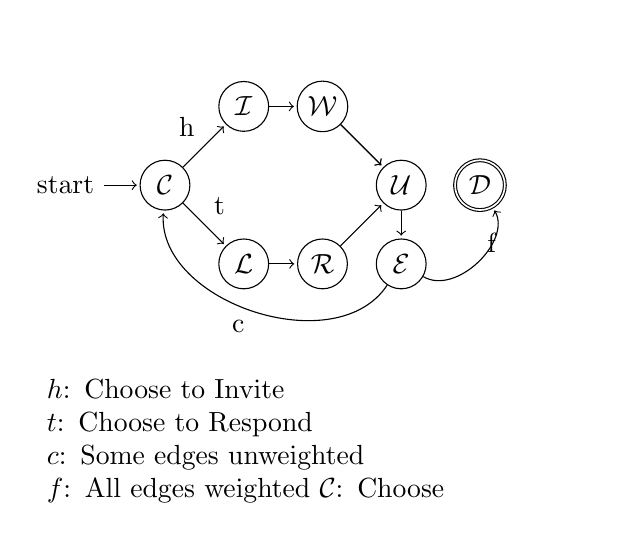
\begin{tikzpicture}[shorten >=1pt,node distance=1cm,on grid,auto, bend angle=75, every state/.style={scale=1, minimum size=18pt, inner sep=2pt}]
    %\draw [help lines] (0,-2) grid (4,2);
    \path [help lines] (0,-2) grid (4,2); 
    \node [state, initial]   (C)          {\cCd};
    \node [state] (I)            at (1,1) {\cId};
    \node [state] (L)            at (1,-1) {\cLd};
    \node [state] (W)            at (2,1)       {\cWd};
    \node [state] (R)            at (2,-1)       {\cRd};
    \node [state] (U)            at (3,0) {\cUd};
    \node [state] (E)            at (3,-1)       {\cEd};
    \node [state, accepting] (D) at (4,0)   {\cDd};

    \path [->] (C) edge              node {h} (I)
                   edge              node {t} (L)
               (L) edge              node {} (R)
               (I) edge              node {} (W)
               (W) edge              node {} (U)
               (R) edge              node {} (U)
               (U) edge              node {} (E);
    \path [->] (E) edge [bend right] node [above right] {f} (D);
    \path [->] (W) edge              node {} (U);
    \path [->] (E) edge [bend left]  node {c} (C);


      \node [text width=7cm] (key) at (2, -3.25) {
	$h$: Choose to Invite \hspace{4cm}
        $t$: Choose to Respond\hspace{4cm}
        $c$: Some edges unweighted\hspace{5cm}
	$f$: All edges weighted
	$\cC$: Choose 
	}; 
  \end{tikzpicture}
  \end{center}
  \label{fig:dgmm-auto}
\end{figure}
  
\end{frame}
\begin{frame}
	\frametitle{Complexity}
	\begin{theorem}
	DGMM solves MWVC to an approximation of two in $O(\Delta)$ rounds with high probability in random graphs.
	\end{theorem}
	\begin{proof}
	\begin{enumerate}
	\item DGMM creates a matching in each round.
	\item A simultaneous weighting of a matching is equivalent to any sequential weighting of that matching.
	\item Approximately $\sfrac{1}{4}$ of a nodes neighbors join the matching in every round.
	\item $\sfrac{1}{2}$ of these are expected to join the cover.
	\item $\approx\sfrac{1}{8}$ of a nodes uncovered edges are covered in each round.
	\end{enumerate}
	\end{proof}
\end{frame}

\begin{frame}
	\frametitle{Redundancy Removal}
	\begin{block}{Algorithm}
	Each node that joins the cover:
	\begin{itemize}
	\item Checks that all of its neighbors are in the cover.
	\item Checks if any of those neighbors are also redundant.
	\item Removes itself from the cover if it is the largest local redundant node.
	\end{itemize}
	\end{block}
\end{frame}

\begin{frame}
  \frametitle{Redundancy Automata}
   \begin{figure}[htp]
  \begin{center}
    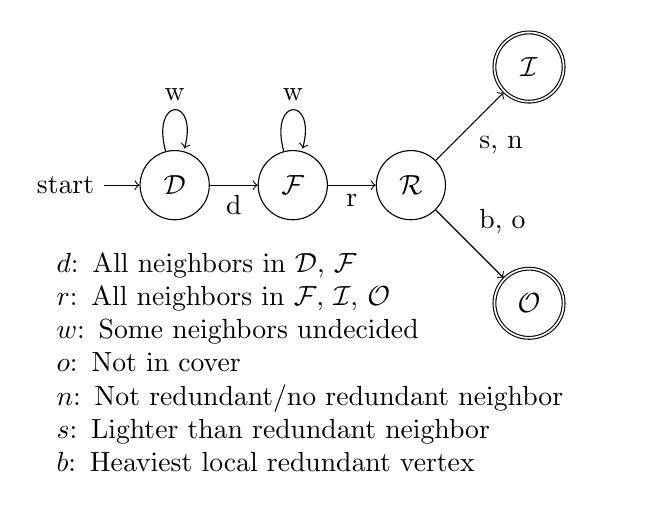
\begin{tikzpicture}
     % \draw[help lines] (0, -2) grid (5,2);
      \path [help lines] (0, -2) grid (5,2);
      \node [state, initial] (D) {\cDd};
      \node [state] (F) at (1.5, 0) {\cFd};
      \node [state] (R) at (3, 0) {\cRd};
      \node [state, accepting] (I) at (4.5, 1.5) {\cId};
      \node [state, accepting] (O) at (4.5, -1.5) {\cOd};

      \path [->] (D) edge node [below] {d} (F)
                     edge [loop above] node {w} ()
                 (F) edge node [below] {r} (R)
                     edge [loop above] node {w} ()
                 (R) edge node [above right]{b, o} (O)
                     edge node [below right]{s, n} (I);
      \node [text width=7cm] (key) at (2, -2.25) {$d$: All neighbors in \cDd, \cFd \hspace{4cm}
        $r$: All neighbors in \cFd, \cId, \cOd  \hspace{4cm}
        $w$: Some neighbors undecided  \hspace{5cm}
        $o$: Not in cover \hspace{5cm}
        $n$: Not redundant/no redundant neighbor  \hspace{4cm}
        $s$: Lighter than redundant neighbor  \hspace{4cm}
        $b$: Heaviest local redundant vertex  \hspace{4cm}};
                     
    \end{tikzpicture}
    \caption{Redundancy Checking Algorithm}
    \label{fig:red}
  \end{center}
\end{figure} 
\end{frame}

\begin{frame}
	\frametitle{Application}
	\begin{block}{MWVC}
	The redundancy removal algorithm had only a modest impact on the size of vertex covers.
	\end{block}
	\begin{block}{Network Lifetime}
	The network lifetime problem benefits from the application of redundancy removal.
	\end{block}
\end{frame}

\section{Network Lifetime}

\begin{frame}
  \frametitle{Network Lifetime}
	\begin{block}{Current Approaches}
	Most approaches to network lifetime rely on a global reshuffle in each round\cite{1640702}. The cost of this reshuffle is usually discounted in evaluation of an algorithm, precisely because of the assumption that all target coverage algorithms require a global reshuffle.
	\end{block}
	\begin{block}{Our Approach}
	We hypothesize that the global reshuffle for a high quality algorithm may cost more than localized reshuffles of a lower quality algorithm. Redundancy checking allows us to asynchronously maintain coverage.
	\end{block}
\end{frame}

\begin{frame}
  \frametitle{Redundancy Checking for Network Lifetime}
	\begin{block}{Algorithm}
	\begin{itemize}
	\item The network is set up initially using any algorithm for target coverage.
	\item When a node in the cover dies, it alerts its neighbors.
	\item The neighbors turn on.
	\item Redundancy checking is used to turn off local redundant neighbors.
	\end{itemize}
	\end{block}
\end{frame}

\section{Experiments}
\begin{frame}
\frametitle{Simulation}
	\begin{block}{Software}
	A generic network simulator was built in Ruby.
	\end{block}
	\begin{block}{Experiments}
	Each algorithm was run against a wide set of degrees and network sizes, and compared to existing approaches to both problems.
	\end{block}
\end{frame}
\begin{frame}[allowframebreaks]
	\frametitle{Results}
	\begin{tiny}
	\begin{figure}[htp]
\begin{center}
\begin{tikzpicture}[scale=.75]
  \begin{axis}[xlabel=Average Degree, ylabel=Total Weight, legend style={at={(.95,.69)}, label={[font=\footnotesize]left:K/Y+R}, font=\footnotesize, anchor=south east}, legend columns=2, cycle list name={four-1-0}]
    \addplot+[grt] table  [x=links, y=star-red]{\averageone};
    \addplot+[grt] table  [x=links, y=star-red]{\averagetwo};
    \addplot+[grt] table  [x=links, y=star-red]{\averagethree};
    \addplot+[grt] table  [x=links, y=star-red]{\averagefour};
    \addplot+[inv] table [x=links, y=mat-red]{\averageone};
    \addplot+[inv] table [x=links, y=mat-red]{\averagetwo};
    \addplot+[inv] table [x=links, y=mat-red]{\averagethree};
    \addplot+[inv] table [x=links, y=mat-red]{\averagefour};
    \legend{(120),(240),(480),(960)}
  \end{axis}
  \begin{axis}[axis x line=none,axis y line=none, legend style={at={(.95,.68)}, label={[font=\footnotesize]left:DGMM+R}, font=\footnotesize, anchor=north east}, legend columns=2, cycle list name={four-0-1}]
    \addplot+[inv] table  [x=links, y=star-red]{\averageone};
    \addplot+[inv] table  [x=links, y=star-red]{\averagetwo};
    \addplot+[inv] table  [x=links, y=star-red]{\averagethree};
    \addplot+[inv] table  [x=links, y=star-red]{\averagefour};
    \addplot+[bls] table [x=links, y=mat-red]{\averageone};
    \addplot+[bls] table [x=links, y=mat-red]{\averagetwo};
    \addplot+[bls] table [x=links, y=mat-red]{\averagethree};
    \addplot+[bls] table [x=links, y=mat-red]{\averagefour};
    \legend{,,,,(120),(240),(480),(960)}
  \end{axis}
\end{tikzpicture}
\caption{Average Weights For MWVC}
\label{plt:mwvc-av}
\end{center}
\end{figure}

	\begin{tikzpicture}[scale=.6]
  \begin{axis}[xlabel=Average Degree, ylabel=Communication Rounds, legend style={at={(0.95,0.95)}, font=\footnotesize, label={[font=\footnotesize]left:K/Y}, anchor=north east}, legend columns=2, cycle list name={four-1-0}]
    \addplot+[grt] table [x=links, y=star-reg]{\runsone};
    \addplot+[grt] table [x=links, y=star-reg]{\runstwo};
    \addplot+[grt] table [x=links, y=star-reg]{\runsthree};
    \addplot+[grt] table [x=links, y=star-reg]{\runsfour};
    \addplot+[inv] table [x=links, y=mat-reg]{\runsone};
    \addplot+[inv] table [x=links, y=mat-reg]{\runstwo};
    \addplot+[inv] table [x=links, y=mat-reg]{\runsthree};
    \addplot+[inv] table [x=links, y=mat-reg]{\runsfour};
    \legend{(120),(240),(480),(960)}
  \end{axis}
  \begin{axis}[axis x line=none, axis y line=none, legend style={at={(0.05,0.425)}, font=\footnotesize, label={[font=\footnotesize]above left:DGMM}, anchor=north west}, legend columns=2, cycle list name={four-0-1}]
    \addplot+[inv] table [x=links, y=star-reg]{\runsone};
    \addplot+[inv] table [x=links, y=star-reg]{\runstwo};
    \addplot+[inv] table [x=links, y=star-reg]{\runsthree};
    \addplot+[inv] table [x=links, y=star-reg]{\runsfour};
    \addplot+[bls] table [x=links, y=mat-reg]{\runsone};
    \addplot+[bls] table [x=links, y=mat-reg]{\runstwo};
    \addplot+[bls] table [x=links, y=mat-reg]{\runsthree};
    \addplot+[bls] table [x=links, y=mat-reg]{\runsfour};
    \legend{,,,,(120),(240),(480),(960)}
  \end{axis}
\end{tikzpicture}


	\begin{figure}[htp]
\begin{center}
\begin{tikzpicture}[scale=.75]
  \begin{axis}[xlabel=Cost, ylabel=Lifetime, legend style={at={(0.05,0.05)}, font=\footnotesize, anchor=south west},  cycle list name={three}]
    \addplot+[bls] table [x=cost, y=deeps_step]{\costcompone};
    \addplot+[bls] table [x=cost, y=deeps_step]{\costcomptwo};
    \addplot+[bls] table [x=cost, y=deeps_step]{\costcompthree};
    \addplot+[inv] table [x=cost, y=deeps_run]{\costcompone};
    \addplot+[inv] table [x=cost, y=deeps_run]{\costcomptwo};
    \addplot+[inv] table [x=cost, y=deeps_run]{\costcompthree};
    \legend{DEEPS (20),DEEPS (40),DEEPS (80)}
  \end{axis}
  \begin{axis}[axis x line=none, axis y line=none, legend style={at={(0.95,0.95)}, font=\footnotesize, anchor=north east},  cycle list name={three}]
    \addplot+[inv] table [x=cost, y=deeps_step]{\costcompone};
    \addplot+[inv] table [x=cost, y=deeps_step]{\costcomptwo};
    \addplot+[inv] table [x=cost, y=deeps_step]{\costcompthree};
    \addplot+[grt] table [x=cost, y=deeps_run]{\costcompone};
    \addplot+[grt] table [x=cost, y=deeps_run]{\costcomptwo};
    \addplot+[grt] table [x=cost, y=deeps_run]{\costcompthree};
    \legend{,,,DEEPS+R (20),DEEPS+R (40),DEEPS+R (80)}
  \end{axis}
\end{tikzpicture}
\caption{Deeps with Communication Costs}
\label{plt:deep-cost}
\end{center}
\end{figure}

	\end{tiny}
\end{frame}
\section{Conclusion}
\begin{frame}
	\frametitle{Conclusions}
	\begin{block}{MWVC}
	Our theory is supported by our experimental results. We believe that we have improved on the prior best known algorithm for MWVC, taking the number of rounds from $\log n$ to $\log \Delta$.
	\end{block}
	\begin{block}{Target Coverage}
	Our experiments suggest that if the cost of global reshuffling is greater than 40\% of the total network maintenance cost, than the local reshuffle approach we present will significantly improve network lifetimes.
	\end{block}
\end{frame}
\begin{frame}
	\frametitle{Future Work}
	\begin{block}{DGMM}
	We intend to improve our DGMM algorithm in two ways:
	\begin{itemize}
	\item Eliminate bad behavior for bad inputs
	\item Extend the approach to the hypergraph
	\end{itemize}
	\end{block}
	\begin{block}{Redundancy}
	Future work for the redundancy algorithm includes:
	\begin{itemize}
	\item Extending this work to the hypergraph
	\item Verifying maintenance cost with physical experiments.
	\end{itemize}
\end{block}
	\end{frame}
\section{Bibliography}
\begin{frame}[allowframebreaks]
\frametitle{Bibliography}
	\bibliography{vertex_bib}
\end{frame}
\end{document}
